\documentclass{ximera}[font=12pt]


\title{Fractions: Multiplication and Division}   % Use xmlatex all -s to compile when SERVE refuses to work.
\author{Kelly Stady}
\license{CC: 0}         % replace with an appropriate license, or set it in xmPreamble

\begin{document}   

\begin{abstract}

\end{abstract}

\maketitle

%\label{xim:FractionsMultDivActivity}


\section*{Multiplying Fractions}

If you have half of a blueberry pie left in the fridge and eat $\textstyle \frac{2}{3}$ \textbf{of} it, what fraction of the \textbf{original whole pie} did you eat?


To eat $\textstyle \frac{2}{3}$ \textbf{of} the half, you would need to divide the half into 3 equal pieces and eat 2 of them.

\begin{center}
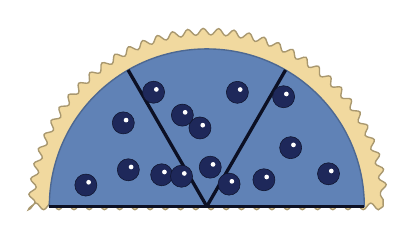
\begin{tikzpicture}[scale=2]   % Blueberry Pie
    % Define colors
    \definecolor{glaucous}{RGB}{96, 130, 182}
    \definecolor{blueberry}{RGB}{30, 40, 90}
    \definecolor{pastry}{RGB}{241, 217, 159}

    % THE CRUST - Semi-circle with fluted edge
    \draw[fill=pastry, draw=pastry!70!black, line width=0.5pt]
          (1.12,0) -- (-1.12,0)
          arc (180:0:1.12) [decoration={snake, amplitude=1.2pt, segment length=5.5pt}, decorate] -- cycle;

    % THE PIE FILLING - Semi-circle
    \draw[fill=glaucous, draw=glaucous!80!black, line width=0.5pt]
          (1.0,0) arc (0:180:1.0) -- cycle;

    % SLICE DIVIDERS - Thick lines matching the whole pie
    \draw[blueberry!40!black, line width=1.2pt] (0,0) -- (60:1.0);
    \draw[blueberry!40!black, line width=1.2pt] (0,0) -- (120:1.0);
    \draw[blueberry!40!black, line width=1.2pt] (1.0,0) -- (-1.0,0); % Flat bottom cut

    % BLUEBERRIES - Exact coordinates from the top half of the whole pie
    \foreach \pos in {
        (135:0.75), (155:0.55), (170:0.78), (145:0.35), (130:0.25), % Upper Left Slice
        (75:0.75), (95:0.5), (115:0.8), (85:0.25), (105:0.6),      % Middle Slice
        (15:0.8), (35:0.65), (55:0.85), (25:0.4), (45:0.2)         % Upper Right Slice
    } {
        \draw[fill=blueberry, draw=blueberry!50!black, line width=0.2pt] \pos circle (0.07);
        \fill[white!90] \pos ++(45:0.025) circle (0.015);
    }

\end{tikzpicture}
%\xmalt{A semi-circle representing the top half of the blueberry pie. The fifteen blueberries are in the exact same positions as the top half of the whole pie illustration.}
\end{center}



If the \textbf{whole} pie was divided into slices of that same size, there would be a total of 6 slices.


\begin{center}
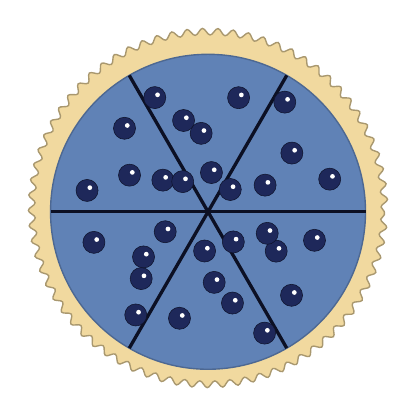
\begin{tikzpicture}[scale=2]
    % Define colors
    \definecolor{glaucous}{RGB}{96, 130, 182}
    \definecolor{blueberry}{RGB}{30, 40, 90}
    \definecolor{pastry}{RGB}{241, 217, 159}

    % THE CRUST - Light golden with wavy fluted edge
    \draw[fill=pastry, draw=pastry!70!black, line width=0.5pt,
          decoration={snake, amplitude=1.2pt, segment length=5.5pt}, decorate] (0,0) circle (1.12);

    % THE PIE FILLING - Glaucous color
    \draw[fill=glaucous, draw=glaucous!80!black, line width=0.5pt] (0,0) circle (1.0);

    % SLICE DIVIDERS - Thicker lines for better visibility
    \foreach \a in {0, 60, 120, 180, 240, 300} {
        \draw[blueberry!40!black, line width=1.2pt] (0,0) -- (\a:1.0);
    }

    % BLUEBERRIES - Adjusted coordinates to clear boundaries
    \foreach \pos in {
        % Upper Left Slice (120 to 180 degrees) - Moved up from mid-lines
        (135:0.75), (155:0.55), (170:0.78), (145:0.35), (130:0.25),
        % Lower Right Slice (300 to 360/0 degrees) - Moved down from mid-line
        (315:0.75), (330:0.5), (345:0.7), (310:0.25), (340:0.4),
        % Other Slices (Restored for full pie)
        (15:0.8), (35:0.65), (55:0.85), (25:0.4), (45:0.2),
        (75:0.75), (95:0.5), (115:0.8), (85:0.25), (105:0.6),
        (195:0.75), (215:0.5), (235:0.8), (205:0.3), (225:0.6),
        (255:0.7), (275:0.45), (295:0.85), (265:0.25), (285:0.6)
    } {
        \draw[fill=blueberry, draw=blueberry!50!black, line width=0.2pt] \pos circle (0.07);
        \fill[white!90] \pos ++(45:0.025) circle (0.015);
    }

\end{tikzpicture}
%\xmalt{A whole blueberry pie with a fluted golden crust and thick slice lines. The glaucous filling is packed with blueberries, all positioned clearly within their slices.}
\end{center}







Since you ate 2 slices, you ate $\textstyle \frac{2}{6}$ or $\textstyle \frac{1}{3}$ of the \textbf{whole} pie.


In mathematics, the word \textbf{of} is code for multiplication.  Therefore, to find $\textstyle \frac{2}{3}$ \textbf{of} $\textstyle \frac{1}{2},$ we multiply the fractions.
To obtain the answer $\textstyle \frac{2}{6}$ mathematically, we would have to multiply the numerators and the denominators.

\begin{align*}
  \frac{2}{3} \textbf{ of } \frac{1}{2} &= \frac{2}{3} \cdot \frac{1}{2} \\
  & \\
  &= \frac{2}{6}
\end{align*}

\begin{procedure}[Multiplying Fractions]

If $a, b, c$ and $d$ are numbers such that $b$ and $d$ are not equal to 0, then

\[ \frac{a}{b} \cdot \frac{c}{d} = \frac{a \cdot c}{b \cdot d} \]


\textbf{In Words:} To multiply fractions, multiply the numerators and the denominators.

\end{procedure}

\begin{remark}
\begin{enumerate}
\item It's a good idea to simplify fractions before multiplying.  If you do so, you
won't have to simplify the answer.

\item Mixed numbers must be written as improper fractions before multiplying.

\item When you multiply a fraction and a whole number, it can be helpful to write the whole
number as a fraction with a denominator of 1.  For example, if you want to find $\textstyle \frac{1}{8}$ \textbf{of} 15, you can write 15
divided by 1 as shown below.

\[ \frac{1}{8} \cdot \frac{15}{1} \]

Now, it's clear which numbers are in the numerator and denominator of each fraction.

\end{enumerate}
\end{remark}

\begin{problem}
Financial advisors recommend spending no more than $\textstyle \frac{3}{10}$ of your monthly take-home pay (your income after taxes and health insurance) on housing costs, like rent or a mortgage.  If your monthly take-home pay is \$2500, what is the maximum amount you should pay for rent or a mortgage?

To determine the maximum amount, find $\frac{3}{10}$ \textbf{of} your monthly take-home pay.

\[ \frac{3}{10} \cdot \frac{2500}{1} = \$ \answer{750} \]

\begin{hint}
It's best to simplify before multiplying.  One way is to divide 2500 by 10, then multiply the result by 3 to get the answer.
\end{hint}

\end{problem}

\end{document}


